The considerations of the previous Section lead to the reasonable
hypothesis that inter-sample distance is the key. Keeping training
sets uniform will result in smaller sets which still contain all
information required for training. Moreover, bad generalisation is
correlated to inter-set distance; therefore uniformisation can be as
well used to retain samples which are far away from the current
training set. We have then implemented an online version of the
uniformisation procedure, in order to test what would happen in a real
setting while the patient is freely moving around.

First of all, since (see Section \ref{subsubsec:electrodes}) the
bandwidth of the EMG signal is limited in our experiment to about
$10$Hz, data have been subsampled from $256$Hz to $25$Hz, getting to a
total training set of about $153,000$ samples. The samples are
naturally chronologically ordered, so that they could be fed to the
system one by one as it would actually happen during continuous
acquisition of data from the patient's activity.

Furthermore, in an online setting no a-priori statistics about the
samples can be assumed. Therefore, as a measure of inter-sample
distance, we dropped the Mahalanobis distance (which requires a good
estimate of the covariance matrix) and resorted to Euclidean distance,
defined in the standard way. Normalisation was still used, as it is
essential for most machine learning methods, but the mean value and
standard deviation of the training sets were evaluated on-the-fly
without keeping the whole sets and re-evaluating them each
time. Testing samples were also normalised according to these
statistics.

(We also tested the batch of samples for dimensionality reduction using
PCA, but found that no more than $2$ or $3$ dimensions could be
eliminated. Therefore we dropped the idea, also since PCA would
require, again, an estimate of the covariance matrix of the data set,
which is not available online.)

The Online Uniformisation (OU) procedure, then, works like this: we
initially fix a minimum inter-sample distance $d$ and start
with an empty training set $S$. Then each time a new sample $\xx$ is
available, we check whether $dist(\xx,\xx_i)\leq d$, for at
least one $\xx_i \in S$: if this is the case, then $\xx$ is discarded;
otherwise, it is added to $S$.

The first question is: does OU give us an acceptable accuracy \emph{at
all times}? That is: does $S$ constitute a good training set, as the
patient explores new regions of the input space, and more and more
samples are seen? In order to answer this question we considered again
the problem of SVM classification, and let $S$ grow according to the
OU procedure. Then, every about $1.5$ minutes of sampled data, that is
every $2,400$ samples, we trained the SVM on $S$ and checked its
accuracy on a testing set drawn from the previously seen samples (but
not in $S$, of course). This was done $5$ times with different splits
of $S$, so to obtain a statistically meaningful measure of
accuracy. We chose to use a mid-range value of $d = 0.21$ obtained
from initial experiments, which would result in a final training set
of about $1800$ samples; moreover, we used hyperparameters $C =
10^{1.5}$ and $\sigma = 10^{0.5}$, found by grid search during the
preliminary experiments. Figure \ref{fig:inc} shows the results.

\begin{figure*}[!ht] \centering
  \begin{tabular}{cc}
    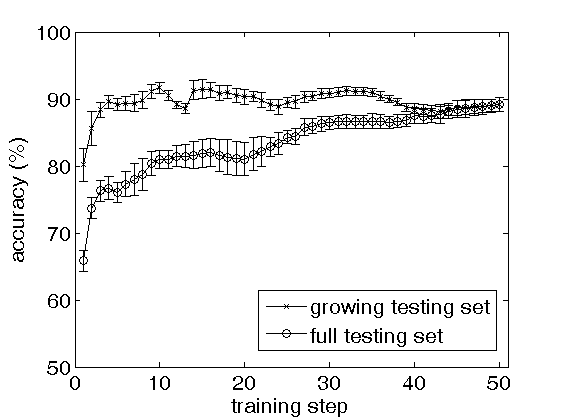
\includegraphics[width=0.45\textwidth]{figs/fig_resInc_OU21.png} &
    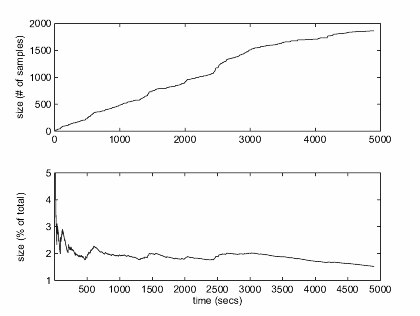
\includegraphics[width=0.45\textwidth]{figs/fig_growth_OU21.png} \\
    $(a)$ & $(b)$ \\
  \end{tabular}
  \caption{$(a)$: classification accuracy of an SVM, as the training set
    grows according to the OU procedure. $(b)$:
    size of the online uniformised training set: number of samples
    (upper plot), fraction of the whole training set (lower plot).}
  \label{fig:inc}
\end{figure*}

Consider first the ``growing testing set'' curve in pane $(a)$ of the
Figure: it is apparent that, already after $4$ training steps, that is
after some $6$ minutes, the system can classify with an accuracy of
about $90\%$, as it was the case in the preliminary analysis (accuracy
$89.57 \pm 0.94$). Notwithstanding some oscillations, the accuracy
remains substantially constant over the whole test and, at the end, is
still $89.14. \pm 1.05$. Consider now the ``full testing set'' curve,
representing the accuracy obtained by the same models but on the
\emph{whole} testing set: now the system is being tested on samples
drawn from zones of the input space it has not yet seen; and, as one
would expect, the accuracy steadily increases, and it finally catches
up with that obtained by testing on the growing testing set.

Consider now pane $(b)$ of the Figure: the upper plot shows the size
of the online uniformised training set as the sample acquisition
proceeds; the lower plot shows the same curve as a fraction of the
full training set size. As time goes on, the OU procedure is letting
the uniform training set grow less and less; the fraction of the full
training set (lower plot) becomes smaller and smaller, being around
$1.5\%$ at the end.

From this we conclude that $(a)$ OU is keeping the training set
remarkably small in absolute terms, and smaller and smaller
percentage-wise, as more and more data is acquired; $(b)$ OU is
``letting in'' only relevant information, since the accuracy is
uniformly high if tested on a growing testing set, and ever growing if
tested upon a full testing set. In other words, the OU procedure is
effective in building a compact and accurate training set for SVM
classification.

As far as other approaches and problems are concerned, Figure
\ref{fig:allres} shows an all-inclusive set of results for all
problems and approaches considered, and for various values of the
minimum distance threshold, $d$, which was fixed at $0.21$ in the
previous experiment.

\begin{figure*}[!ht] \centering
  \begin{tabular}{cc}
    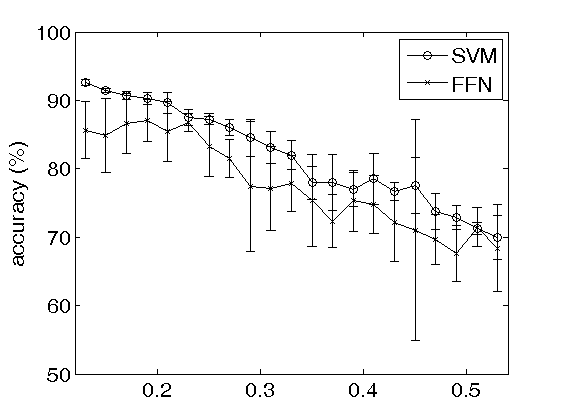
\includegraphics[width=0.45\textwidth]{figs/fig_all1.png} &
    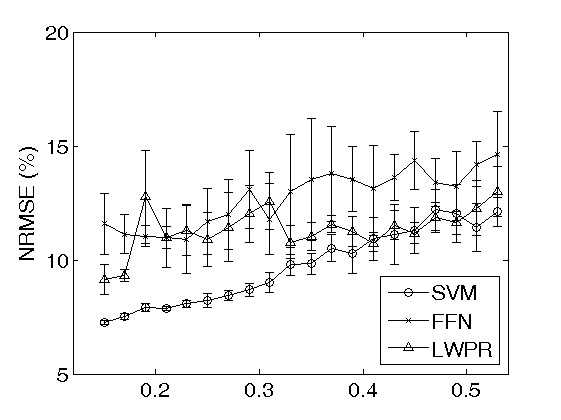
\includegraphics[width=0.45\textwidth]{figs/fig_all2.png} \\
    $(a)$ & $(b)$ \\
  \end{tabular}
  \caption{Classification and regression results using the OU
  procedure, as $d$ is increased. $(a)$: classification, $(b)$:
    regression. Compare with Figure \ref{fig:TSsize} for the training
    set sizes.}
  \label{fig:allres}
\end{figure*}

As $d$ is increased from $0.13$ to $0.53$, all approaches show a
decreasing performance, as expected: in classification, the SVM is
uniformly better, going from $92.61\%$ for $d=0.13$ to $70.01\%$ for
$d=0.53$. The standard deviations for the SVM are, also, uniformly
smaller. In regression, again, the SVM is uniformly better than the
other approaches, ranging from $7.09\%$ NRMSE to $12.12\%$, and it
also shows uniformly smaller standard deviations. In both problems,
however, it must be remarked that the error bars largely overlap, at
least for $d>0.4$ for regression. This enables us to conclude that the
SVM is the winning approach overall, but that there are cases in which
another approach can be better.

One last consideration: as $d$ is increased, the size of the training
sets decreases like $d^{-10}$, since we are building a finite
partitioning of a subset of $\RR^{10}$ (see also Figure
\ref{fig:TSsize}, in which the training set size is plotted as a
function of $d$); whereas, it seems that the accuracy of all
approaches, and in both problems, only decreases linearly. This is a
remarkable feature of the OU procedure, since it will always be
possible to choose a $10$-degree polynomially smaller training set and
obtain a machine which is only linearly worse.

\begin{figure}[!ht] \centering
  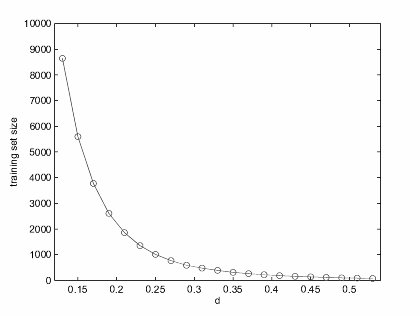
\includegraphics[width=0.45\textwidth]{figs/fig_allSize.png} \\
  \caption{Online uniformised training set size as $d$ changes.}
  \label{fig:TSsize}
\end{figure}

As a matter of fact, consider once again Figure \ref{fig:allres}, pane
$(b)$: at the far right end we have a SVM which has a still acceptable
error of $12.12\% \pm 0.64\%$, but whose training set, averaged over
the $5$ splits, consists of $77.4$ samples out of the original
$153000$!

Lastly, we compared the results obtained by models trained on uniform
training sets with a simple random selection strategy. In this case,
rather than employing the OU procedure to reduce the training sets,
for each value of $d$ we chose at random the same number of samples
obtained by the OU procedure, and then trained on the models so
obtained. It was expected that, on full training sets, the random
strategy would outperform OU; this is due to the fact that a random
strategy will result in training sets which have the same probability
distribution as the full testing sets; whereas, the OU procedure
produces training sets with a uniform probability distribution. The OU
procedure, on the other hand, is expected to perform better on
\emph{uniform testing sets}, for the same reason. Figure
\ref{fig:rnVSuni} shows the comparative results for SVM classification
and regression, confirming our expectations.

\begin{figure*}[!ht] \centering
  \begin{tabular}{cc}
    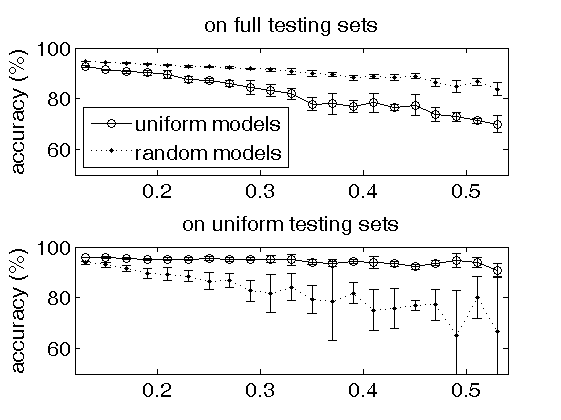
\includegraphics[width=0.45\textwidth]{figs/fig_rnVSuni1.png} &
    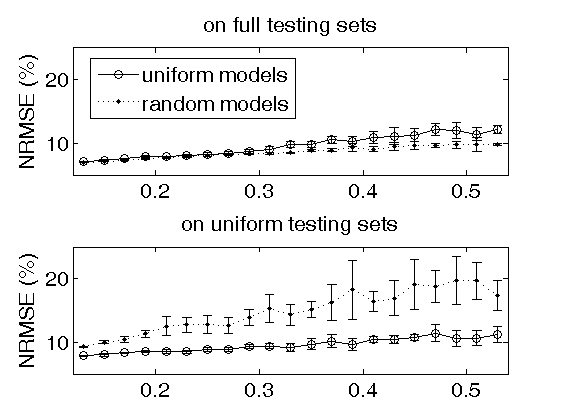
\includegraphics[width=0.45\textwidth]{figs/fig_rnVSuni2.png} \\
    $(a)$ & $(b)$ \\
  \end{tabular}
  \caption{Classification and regression results, comparing the OU
  procedure with a random sample selection strategy. $(a)$:
    classification, $(b)$: regression.}
  \label{fig:rnVSuni}
\end{figure*}

As one can see, both in classification and in regression, an SVM
trained on uniform training sets will perform uniformly better than
one trained on random training sets, when tested on uniform testing
sets; and uniformly worse when tested on the full training sets. But
the gap is larger in favour of the uniform training sets. This lets us
conclude that uniform training sets will produce models able to
perform \emph{uniformly well} in all situations the patient should
move. This is very useful in a practical setting: for example, picture
a seldom performed movement, such as turning a door handle; if we were
employing random training sets, we would have a much worse performance
on such a movement. Uniform training sets would make the patient's
life easier.
